\documentclass[12pt]{article}

\title{The Standard Control Framework}
\author{Samir Menon}

\usepackage{graphicx}
\usepackage[top=2cm, bottom=3cm, left=1.5cm, right=1.5cm]{geometry}
\usepackage{tabularx} %For stretching tables.
\usepackage{verbatim} %For multi-line \begin{comment}
\usepackage{fancyvrb} %For verbatim footnotes
\VerbatimFootnotes

\begin{document}
\maketitle

This document describes the development of a novel force-control and dynamic simulation 
framework. The framework, developed in C++, is a loose collection of modules
that can run a dynamics simulation for articulated bodies, control it, and also
render it graphically. 
It contains standard APIs for the necessary modules, and provides default 
implementations for each API (Fig. \ref{fig:scf}). 
Its various APIs, their implementations and other components are:

\begin{enumerate}
 \item A Control API
    \begin{enumerate}
      \item The Standard Control Library
    \end{enumerate}
 \item A Rigid Body Dynamics API
    \begin{enumerate}
      \item The Tao dynamics engine (kinematics, and forward and inverse dynamics algorithms)
      \item Interfaces to Real Robots (forward dynamics)
    \end{enumerate}
 \item A Graphics API
    \begin{enumerate}
      \item The Chai graphics engine
    \end{enumerate}
 \item A File Parsing API
    \begin{enumerate}
      \item The Lotus XML file format parser
      \item The SAI XML file format parser
      \item The OpenSim XML file format parser
      \item The Lotus yaml file format parser
    \end{enumerate}
  \item Data structures for shared memory between modules
  \item Callbacks for message passing between modules
  \item Helper functions for calling the APIs through an easy to use, 
high level interface
\end{enumerate}

Any standard application may use one or more of the above modules. A full robot 
dynamics simulation will typically use all of them, and might add specific controller
and callback extensions.

\begin{figure}
\begin{center}
\includegraphics{figs/scf.pdf}
\end{center}
\caption{The Lotus Controller and Simulator, the Standard Control Framework, and 
commonly used third party libraries. Typical applications like Lotus, will link with
scf and the third parties and also add their own code to customize user interaction.}
\label{fig:scf}
\end{figure}

\section{The Control API}

The control API enables a dual-rate dynamic force-controllers, where a fast servo
loop computes actuator forces and torques, while a possibly slower model update loop
computes the dynamic state f the articulated rigid body system (Fig. \ref{fig:scl}). 
Our default implementations of this API is:

\begin{figure}[t!]
\begin{center}
\includegraphics[width=7in]{figs/controller.pdf}
\end{center}
\caption{The Standard Control Library's two-stage task space control architecture.}
\label{fig:scl}
\end{figure}

\subsection{SCL : The Standard Control Library}
The SCL contains two types of controllers to meet the APIs requirements
\begin{description}
  \item{\bf Generalized Coordinate Control:} The generalized coordinate (gc) controller
takes the state of the robot, a gc trajectory and uses a dynamic model to compute
actuator control forces. For robots, which are typical articulated rigid body systems,
the gc controller generates joint torques.

  \item{\bf Task Space Control:} The task space controller implements a prioritized 
multi-level task control strategy that takes multiple tasks, arranges them so that lower
priority tasks operate in the null space of higher priority tasks, and finally sums
the gc forces that each task generates within its range space. Our task control 
implementation also includes common operational space control tasks such as 
operational point position, frame orientation, and null space control. 

The tasks are easily specified in an xml file, and typical controllers may be built
without writing any C++ code.
\end{description}

\section{The Rigid Body Dynamics API}
The rigid body dynamics API serves two functions. First to compute the forward dynamics,
which involves soving the physics equations of motion for articulated rigid bodies. And
second to compute various kinematic and dynamic quantities like kinematic 
transformations, Jacobian matrices, generalized inertia matrices etc.

\subsection{The Tao Dynamics Library}
Our default implementation of the dynamics API is Tao. Tao is an open source library
released under the MIT license and provides forward and inverse dynamics algorithms
along with algorithms to compute the kinematic transformations and Jacobians.

\subsection{Interfaces to Robots}
Monitoring a real robot's physical motion can be a substitute for solving forward
dynamics equations. We are presently working on providing interfaces to the Kuka
Lightweight Arm, the Puma robot, and the Pr2 robot.

\section{The Graphics API}
The graphics API provides basic functions to render a set of rigid and articulated
bodies. Essentially, it implements a scene graph of articulated and rigid bodies, and
uses some underlying graphics implementation (like OpenGL) to render them.
It also computes contacts between different graphical objects, and sends them
to the dynamics engine for contact resolution.

\subsection{The Chai3d Graphics}
The default graphics implementation we use is called Chai3d. Please see ``http://www.chai3d.org/'' for more details.

\section{The Parser API}
Since there may be multiple API implementations for the other modules, we decided
to standardize a {\em file format independent} parser API that could allow each module
to maintain a specific file format, and at the same time provide a clean interface to
wrap all the module file formats together. This has allowed us to simultaneously 
support multiple file formats:

\subsection{Lotus XML}
The lotus XML is the most general of our implementations, and provides xml parsing
for all the default module implementations.
\begin{description}
  \item {\bf World: } This allows specifying global physical properties such as gravity
  \item {\bf Robot: } This allows specifying one or more robots in a tree-like 
branching structure. The robot links are arranged in flat (not recursive) xml tags. Ie.
the links are all at the same level in an xml schema, and are arranged into a tree
by name and parent name tags at the time of parsing.
  \item {\bf Graphics: } This allows specifying non-physics objects, lighting, and 
cameras.
  \item {\bf Controller: } This allows specifying one or more controllers and their tasks.
\end{description}

Since almost every static parameter can be specified in the file format, writing code
is only required for dynamic user interaction.

\subsection{SAI XML}
We provide legacy file format parsing to convert older SAI XML into Lotus XML.

\subsection{OpenSim XML}
We also provide file format parsing to convert the biomechanics OpenSim XML file format
into Lotus XML.

\subsection{Lotus Yaml}
We also plan to support a file format based on yaml. Yaml has numerous advantages over
xml because it is usually more compact, expressive, easily readable and can also serve
as a serialized format for message passing.

\section{Shared Memory}
The primary method for modules to share information with each other is shared memory,
implemented through a shared data structure singleton called the Database. 

\section{Message Passing}
As an alternative to accessing shared memory, we also support a set of statically 
defined callbacks. The advantage of using template based static callbacks, against 
using dynamic callbacks using virtual functions, is that our code is more modular,
cleaner, and much faster.

\section{Helper functions and classes}
While the scf exposes its api at a very low level and is primarily geared towards
advanced users, most users prefer a simpler high-level interface. To meet their needs,
we also support a Robot API, a collection of high-level helper functions and
classes that can help quickly build an application.


\end{document}


